
\section{The Visualizer}

From the learnings in the first simulations using the Python based
NS-3 API the second part of the project includes the development of
a network visualizer in C++. The architectual principles as described
in chapter \ref{sub:Architecture} also apply to the C++ based API.
Actually the Python based API of NS-3 is a 1:1 mapping of C++ classes
to Python classes using the pybindgen Framework.


\subsection{Dual Hop network visualization}

The main program of the C++ based visualizer is very similar to the
Python based application but ported to C++. Similar to the procedures
in the Python based simulations the first C++ based simulation included
the implementation of a network visualization using only three nodes
as shown in Figure \ref{fig:Point-To-Point-connection-between}. In
addition to the Python based simulations now the simulation includes
real Wifi channels between the nodes instead of simple Point-To-Point
connections. The relevant Wifi initialization is shown in Listing
\ref{lst:wifi_initialization}.

\texttt{\small \lstinputlisting[breaklines=true,caption={wifi-project.cc (wifi initialization)},extendedchars=true,firstline=52,label={lst:wifi_initialization},language={C++},lastline=63,numbers=right]{src/wifi-project/wifi-project.cc}}{\small \par}

Again we generate pcap based trace files (line 61). Furthermore NS-3
helper objects are being used (lines 57-58) to initialize a {}``default''
Wifi model to our simulation. The NS-3 documentation does not clearly
state what the default settings are, so there was some investigation
necessary. Listing \ref{lst:wifilog} shows the log output from the
NS-3 Wifi helper classes. It can be seen that there are pretty lots
of meaningless pointer values in hex format. The only valuable information
is that the Wifi connection has a speed of 6MBit. Clearly this is
a point for enhancement in NS-3 since neither the documentation states
what the default Wifi values are nor the log output (which also has
to be enabled separately). Of course these settings can be programmatically
controlled using the C++ API but the investigation of different Wifi
propagation settings was not part of this project.

\texttt{\small \lstinputlisting[breaklines=true,caption={wifilog.out (log output from NS-3 Wifi helper objects)},extendedchars=true,firstline=1,label={lst:wifilog},lastline=43,numbers=right]{src/results/wifilog.out}}{\small \par}

Since we want to visualize the nodes we have to decide on a positioning
model. NS-3 supports a three-dimensional model using a x-y-z axis
for physically placing nodes. A three-dimensional visualization is
possible using 3D based APIs and there is also a plugin in development
for 3D based NS-3 visualization, but the goal was to implement a similar
visualization to the OLPC flash version as show in Figure \ref{fig:OLPC-network-visualization}
which is clearly based on a simple two-dimensional pane. Therefore
all z-Values were left zero. Listing \ref{lst:dualhop_pos_initialization}
shows the initialization of the physical positions of the three nodes.
The code can be interpreted as follows:
\begin{itemize}
\item line 101: position all nodes on a grid
\item line 102: The minimum x and y location is 10 meters away from the
corner of the simulated pane
\item line 103: The distance between the nodes equals the variable {}``distance'',
which in our case is 100 meters.
\item line 104: The layout type is {}``row first''. That means that the
nodes are being placed automatically in a row first and then, if there
is no place left, one column up.
\end{itemize}
\texttt{\small \lstinputlisting[breaklines=true,caption={wifi-project.cc (position initialization)},extendedchars=true,firstline=99,label={lst:dualhop_pos_initialization},language={C++},lastline=106,numbers=right]{src/wifi-project/wifi-project.cc}}{\small \par}

Similar to the Python based simulations an application logic had to
be implemented. Instead of using built-in NS-3 helper objects an own
application was implemented called wifi-trace which sends UDP packets
every n seconds to the client. The idea was to have bursts of packets
every n seconds which then can be visualized. The relevant sending
logic can be seen in Listing \ref{lst:wifi_trace_sender}.

\texttt{\small \lstinputlisting[breaklines=true,caption={wifi-trace-apps.cc (sender application logic)},extendedchars=true,firstline=115,label={lst:wifi_trace_sender},language={C++},lastline=140,numbers=right]{src/wifi-project/wifi-trace-apps.cc}}{\small \par}

Now in order to visualize a packet route single hops of the packets
traveling through the network have to be catched. NS-3 has a built-in
mechanisms for so called callbacks. Dedicated listener objects can
then be instanciated and can be hooked to listen to callback methods.
Such a listener was implemented in this project and called PacketListener
(defined in packet-listener.cc/packet-listener.h). The callbacks defined
in this project can be seen in Listing \ref{lst:callback_init_}.

\texttt{\small \lstinputlisting[breaklines=true,caption={wifi-project.cc (callback initialization)},extendedchars=true,firstline=133,label={lst:callback_init_},language={C++},lastline=136,numbers=right]{src/wifi-project/wifi-project.cc}}{\small \par}

In Listing \ref{lst:callback_init_} the following two callback methods
are initialized:
\begin{itemize}
\item \textit{Sender}: Whenever a new packet is being transmitted by the
sender application the listener has to be notified about this fact.
The method being triggered is called PacketListener::TxCallback as
shown in Listing \ref{lst:tx_callback}. The listener then stores
the id of the packet in a hashmap (line 66) and knows that a new transmission
is starting.
\item \textit{In-between hop nodes}: Whenever a node is being used as a
router by the OLSR protocol in order to forward a packet to its destination
then the listener has to be notified about this fact. The method being
triggered here is called PacketListener::RxCallback as shown in Listing
\ref{lst:rx_callback_}. The connection of the current node and the
previous node (line 116) can then be drawn as a part of the whole
routing graph in the visualization.
\end{itemize}
\texttt{\small \lstinputlisting[breaklines=true,caption={packet-listener.cc (TxCallback)},extendedchars=true,firstline=64,label={lst:tx_callback},language={C++},lastline=70,numbers=right]{src/wifi-project/packet-listener.cc}}{\small \par}

\texttt{\small \lstinputlisting[breaklines=true,caption={packet-listener.cc (RxCallback)},extendedchars=true,firstline=103,label={lst:rx_callback_},language={C++},lastline=118,numbers=right]{src/wifi-project/packet-listener.cc}}{\small \par}

The visualized packet route is not displayed in realtime during the
simulation but rather logged to a special file. This file is being
interpreted by a newly available NS-3 plugin called {}``Decorator
API'' . The result of the dual-hop visualization can be seen in
Figure \ref{fig:Dual-Hop-visualization}. The pink line represents
an UDP packet travelling via all intermediate nodes forming a route
graph.

%
\begin{figure}
\begin{centering}
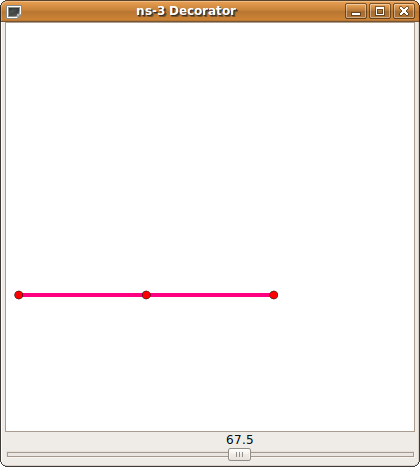
\includegraphics[scale=0.5]{src/results/dualhop_visualization}
\par\end{centering}

\caption{\label{fig:Dual-Hop-visualization}Dual Hop visualization}



\end{figure}



\subsection{Grid network visualization}

Based on the learnings from the Dual Hop visualization and the first
Pyhton based simulations now the final goal was to implement a visualization
of a grid of nodes. It was assumed that the lowest left-most node
is the sender node. Then a receiver node is walking across a grid
of other nodes starting from the middle of the pane. It was assumed
that due to the nature of the OLSR protocol the route graph would
then adapt itself targetting the current position of the walking node.
The distance between all nodes was set up to 100 meters so there was
no danger of a direct connection between the sender and the receiver
node because the distance would be too far.

Listing \ref{lst:grid_network} shows the central simulation code
for the grid simulation. Lines 146-163 initialize the target nodes.
One can see, that a total of 17 nodes is being created. 16 nodes a
are forming a 4x4 grid. The 17th node is the walking node. Lines 169-190
initilialize the mobility model of the 16 grid nodes. The following
properties were programmed for the grid nodes:
\begin{itemize}
\item \textit{Grid positions}: The grid nodes are placed in a grid. A helper
object called ns3::GridPositionAllocator was used to achieve the grid
layout.
\item \textit{Constant positiions}: The grid nodes are node supposed to
move. Therefore a helper object called ns3::ConstantPositionMobilityModel
was used to initalize the grid nodes.
\end{itemize}
Afterwards the moving node is being initialized with the following
properties:
\begin{itemize}
\item Middle start position: The walking node starts from the middle of
the grid pane. Lines 192-195 specify the concrete x-y start position.
\item Random walking: The walking node randomly walks inside the grid. Lines
197-199 specify the random walk model using a helper object called
ns3::RandomWalk2dMobilityModel.
\end{itemize}
Lines 204-208 initialize the Decorator API to be able to visualize
the routing graph. Lines 211-222 initialize the sender and receiver
application. Lines 224-226 initialize the already describe packet
listener. Finally the already discussed callbacks are being initialized
and the simulation starts.

\texttt{\small \lstinputlisting[breaklines=true,caption={wifi-project.cc (grid simulation)},extendedchars=true,firstline=146,label={lst:grid_network},language={C++},lastline=243,numbers=right]{src/wifi-project/wifi-project.cc}}{\small \par}

%
\begin{figure}
\hfill{}\subfloat[53.4th second]{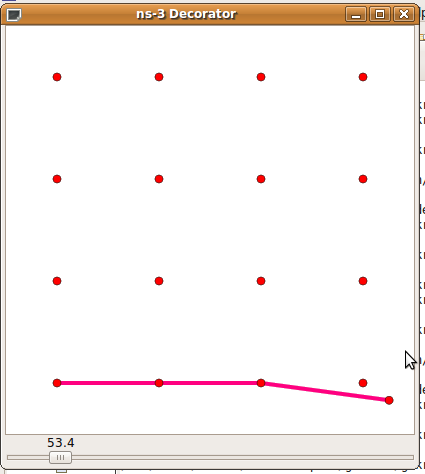
\includegraphics[scale=0.3]{src/results/Screenshot}



}\hfill{}\subfloat[130.4th second]{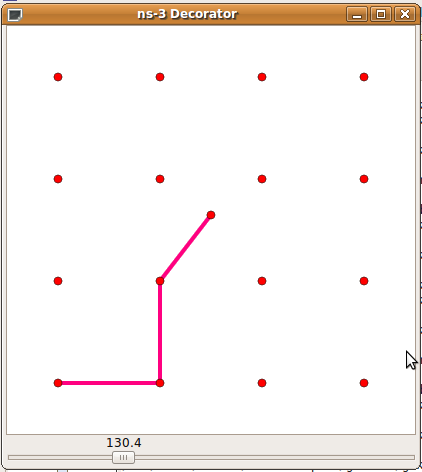
\includegraphics[scale=0.3]{src/results/Screenshot-1}

}\hfill{}

\hfill{}\subfloat[207.4th second]{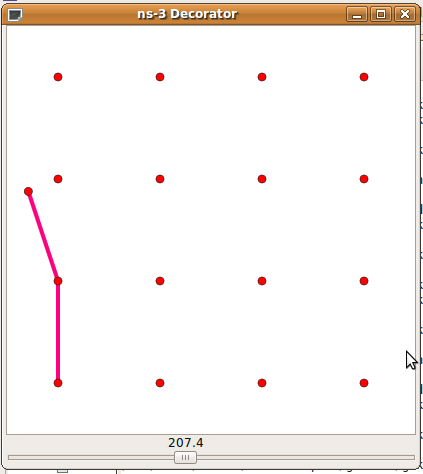
\includegraphics[scale=0.3]{src/results/Screenshot-2}

}\hfill{}\subfloat[263.3th second]{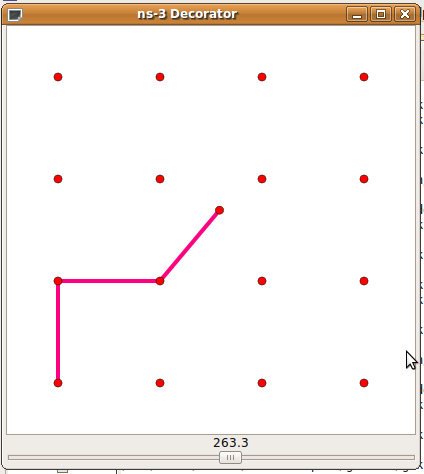
\includegraphics[scale=0.3]{src/results/Screenshot-3}

}\hfill{}

\hfill{}\subfloat[319.1th second]{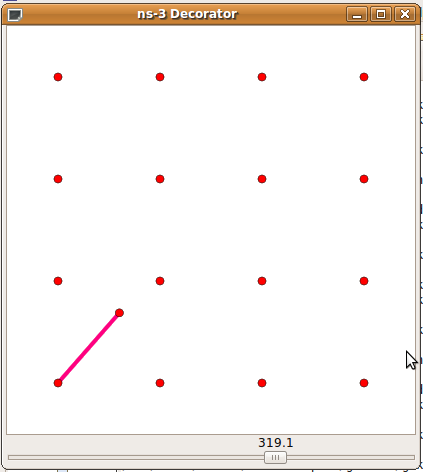
\includegraphics[scale=0.3]{src/results/Screenshot-4}

}\hfill{}\subfloat[408.5th second]{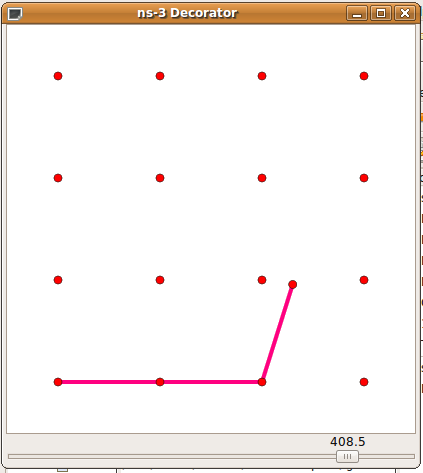
\includegraphics[scale=0.3]{src/results/Screenshot-5}

}\hfill{}

\hfill{}\subfloat[445.8th second]{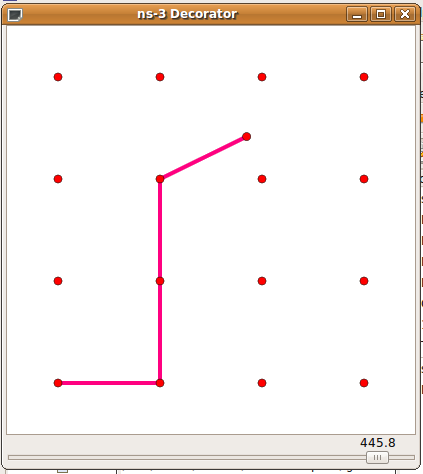
\includegraphics[scale=0.3]{src/results/Screenshot-6}

}\hfill{}\subfloat[466.9th second]{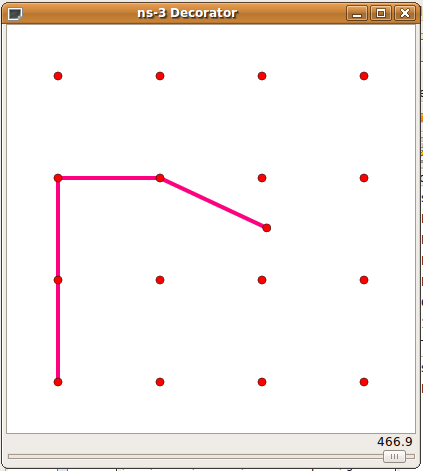
\includegraphics[scale=0.3]{src/results/Screenshot-7}

}\hfill{}

\caption{\label{fig:The-grid-network}The grid network visualization}



\end{figure}


Figure \ref{fig:The-grid-network} shows single snapshops of the overall
visualized simulation at different time points. One can see how the
receiver node walks randomly amongst the grid of router node.
